\usepackage{tikz}

% 1. Definición de colores
\definecolor{lightcyan}{RGB}{220, 248, 248}
\definecolor{lightpink}{RGB}{214, 126, 161} % Ajustado ligeramente al tono de la imagen

% 2. Configuración de estilos globales para el diagrama
\tikzset{
    box_base/.style={rectangle, rounded corners, minimum height=2.2cm, text centered, draw=black, thick},
    box_phrase/.style={box_base, fill=lightcyan, minimum width=2.5cm},
    box_step/.style={box_base, fill=lightpink, minimum width=2cm},
    arrow/.style={thick,->,>=stealth}
}

% 3. CREACIÓN DEL COMANDO
% Todo lo que está dentro de este comando se dibujará cuando lo llames.
% 3. Definición del comando
\newcommand{\embeddingflujo}{%
    \begin{tikzpicture}[
        >=latex,
        node distance=0.8cm,
        inp/.style={draw, thick, fill=purple!50, rounded corners=3pt, minimum width=2.6cm, minimum height=1.5cm, align=center},
        tok/.style={draw, thick, fill=purple!50, rounded corners=3pt, minimum width=2.8cm, minimum height=1.5cm, align=center},
        emb/.style={draw, thick, fill=teal!50, rounded corners=3pt, minimum width=2.8cm, minimum height=1.5cm, align=center},
        trans/.style={draw, thick, fill=orange!40, rounded corners=3pt, minimum width=2.8cm, minimum height=1.5cm, align=center},
        arrow/.style={thick, ->}
    ]
        
        % 1. Nodo Frase
       \node (frase) [align=center] {El gato está \\ sobre la mesa};

        % 2. Nodo Tokenizador (con los corchetes protegidos por llaves {})
        \node (tokenizer) [tok, right=of frase] 
            { Tokenizador \\ {[$id_1, id_2, \dots$]}};

        % 3. Nodo Embedding
        \node (embedding) [emb, right=of tokenizer] { \textit{Embedding} \\ $\{ x_1, x_2, \dots \}$};

        % 4. Nodo Transformador (eliminado el 'at' incorrecto)
        \node (transformer) [trans, right=of embedding] { Transformador };

        % 5. Nodo Output (añadida posición a la derecha del transformador)
        \node (output) [right=of transformer] {$\mathbf{Y}$};

        % Conexiones
        \draw [arrow] (frase) -- (tokenizer);
        \draw [arrow] (tokenizer) -- (embedding);
        \draw [arrow] (embedding) -- (transformer);
        \draw [arrow] (transformer) -- (output);
        
    \end{tikzpicture}%
}

%===========================
%DECODIFICADOR
%===========================
\newcommand{\DiagramaDecodificador}{
    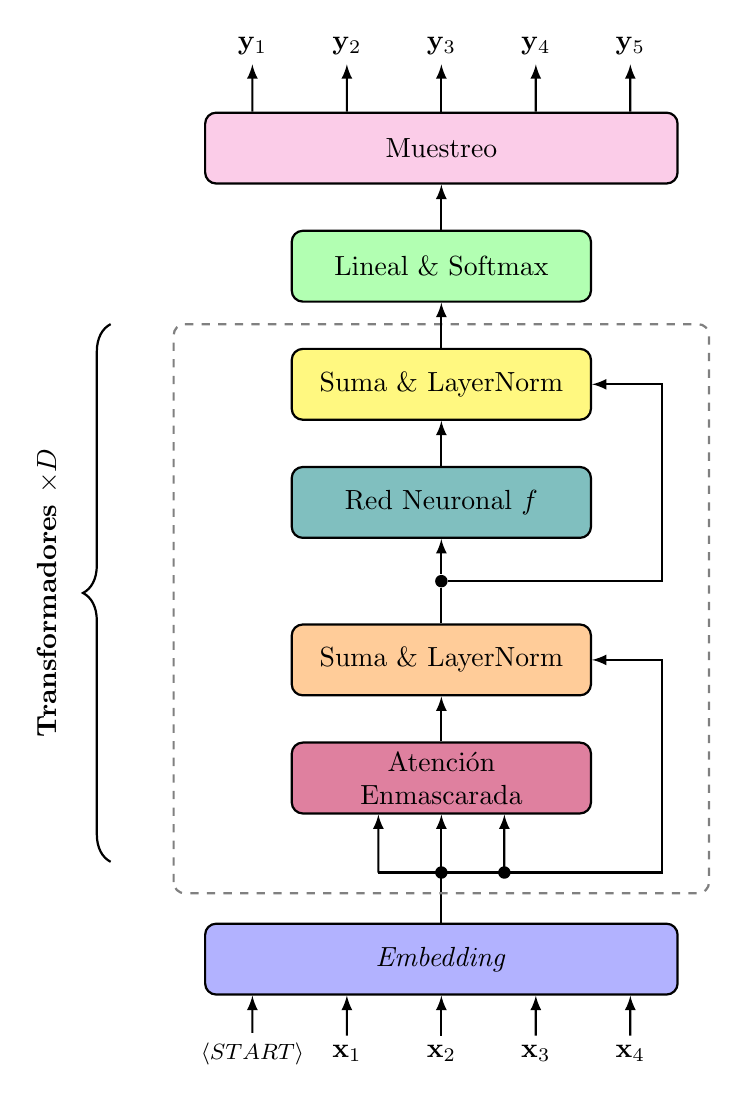
\begin{tikzpicture}[
        >=latex,
        box/.style={
            draw, thick, rounded corners=4pt, 
            minimum width=6cm, minimum height=0.9cm, 
            align=center
        },
        % Estilos de los bloques
        emb/.style={box, fill=blue!30},
        attn/.style={box, fill=purple!50, minimum width=3.8cm},
        addnorm/.style={box, fill=orange!40, minimum width=3.8cm},
        mlp/.style={box, fill=teal!50, minimum width=3.8cm},
        final/.style={box, fill=yellow!50, minimum width=3.8cm},
        outbox/.style={box, fill=green!30, minimum width=3.8cm},
        ybox/.style={box, fill=magenta!20, minimum width=6cm}, % Misma anchura que Embedding
        dot/.style={circle, fill=black, inner sep=0pt, minimum size=4.5pt}
    ]
    
    % 1. ENTRADAS (Tokens)
    \node[font=\footnotesize] (x_0) at (-2.4, 0) {$\langle START \rangle$};
    \node (x_1) at (-1.2, 0) {$\mathbf{x}_1$};
    \node (x_2) at (0, 0) {$\mathbf{x}_2$};
    \node (x_3) at (1.2, 0) {$\mathbf{x}_3$};
    \node (x_4) at (2.4, 0) {$\mathbf{x}_4$};
    
    % 2. BLOQUE EMBEDDING
    \node[emb] (emb) at (0, 1.2) {\textit{Embedding}};
    
    \draw[->, thick] (x_0) -- ([xshift=-2.4cm]emb.south);
    \draw[->, thick] (x_1) -- ([xshift=-1.2cm]emb.south);
    \draw[->, thick] (x_2) -- (emb.south);
    \draw[->, thick] (x_3) -- ([xshift=1.2cm]emb.south);
    \draw[->, thick] (x_4) -- ([xshift=2.4cm]emb.south);
    
    % 3. Bifurcación de entrada al Transformer
    \coordinate (c_center) at (0, 2.3);
    \coordinate (c_left) at (-0.8, 2.3);
    \coordinate (c_right) at (0.8, 2.3);
    
    \draw[thick] (emb.north) -- (c_center);
    \draw[thick] (c_center) -- (c_left);
    \draw[thick] (c_center) -- (c_right);
    \node[dot] at (c_center) {};
    \node[dot] at (c_right) {};
    
    % 4. BLOQUE DE ATENCIÓN
    \node[attn] (mha) at (0, 3.5) {Atención \\ Enmascarada};
    \draw[->, thick] (c_center) -- (mha.south);
    \draw[->, thick] (c_left) -- ([xshift=-0.8cm]mha.south);
    \draw[->, thick] (c_right) -- ([xshift=0.8cm]mha.south);

    % 5. PRIMER ADD & NORM
    \node[addnorm] (an1) at (0, 5.0) {Suma \& LayerNorm};
    \draw[->, thick] (mha.north) -- (an1.south);
    \draw[->, thick] (c_right) -- (2.8, 2.3) |- (an1.east);
    
    % 6. PUNTO INTERMEDIO Z
    \coordinate (z_pos) at (0, 6.0);
    \node[dot] (dot_z) at (z_pos) {};
    \draw[thick] (an1.north) -- (dot_z);
    
    % 7. BLOQUE MLP
    \node[mlp] (mlp) at (0, 7.0) {Red Neuronal $f$};
    \draw[->, thick] (dot_z) -- (mlp.south);
    
    % 8. SEGUNDO ADD & NORM
    \node[final] (an2) at (0, 8.5) {Suma \& LayerNorm};
    \draw[->, thick] (mlp.north) -- (an2.south);
    \draw[->, thick] (dot_z) -- (2.8, 6.0) |- (an2.east);

    % --- RECUADRO DISCONTINUO ---
    \draw[dashed, thick, gray, rounded corners=4pt] 
        ([xshift=-3.4cm, yshift=-1cm]mha.south) 
        rectangle 
        ([xshift=3.4cm, yshift=0.3cm]an2.north);
        
    % --- LLAVE IZQUIERDA ---
    \draw[decorate, decoration={brace, amplitude=10pt}, thick] 
        ([xshift=-4.2cm, yshift=-0.6cm]mha.south) -- 
        ([xshift=-4.2cm, yshift=0.3cm]an2.north) 
        node[midway, xshift=-0.8cm, rotate=90, font=\bfseries] {Transformadores $\times D$};

    % 9. CAPA LINEAL & SOFTMAX
    \node[outbox] (soft) at (0, 10.0) {Lineal \& Softmax};
    \draw[->, thick] (an2.north) -- (soft.south);
    
    % 10. NUEVA CAJA DE SALIDA (Tipo Embedding)
    \node[ybox] (y_box) at (0, 11.5) {Muestreo};
    \draw[->, thick] (soft.north) -- (y_box.south);

    % 11. VECTORES DE SALIDA y_1 a y_5
    \node (y_1) at (-2.4, 12.8) {$\mathbf{y}_1$};
    \node (y_2) at (-1.2, 12.8) {$\mathbf{y}_2$};
    \node (y_3) at (0, 12.8) {$\mathbf{y}_3$};
    \node (y_4) at (1.2, 12.8) {$\mathbf{y}_4$};
    \node (y_5) at (2.4, 12.8) {$\mathbf{y}_5$};

    % Flechas desde la caja hacia los vectores y
    \draw[->, thick] ([xshift=-2.4cm]y_box.north) -- (y_1);
    \draw[->, thick] ([xshift=-1.2cm]y_box.north) -- (y_2);
    \draw[->, thick] (y_box.north) -- (y_3);
    \draw[->, thick] ([xshift=1.2cm]y_box.north) -- (y_4);
    \draw[->, thick] ([xshift=2.4cm]y_box.north) -- (y_5);
    
    \end{tikzpicture}
}



%===========================
%CODIFICADOR
%===========================
\newcommand{\DiagramaCodificador}{
    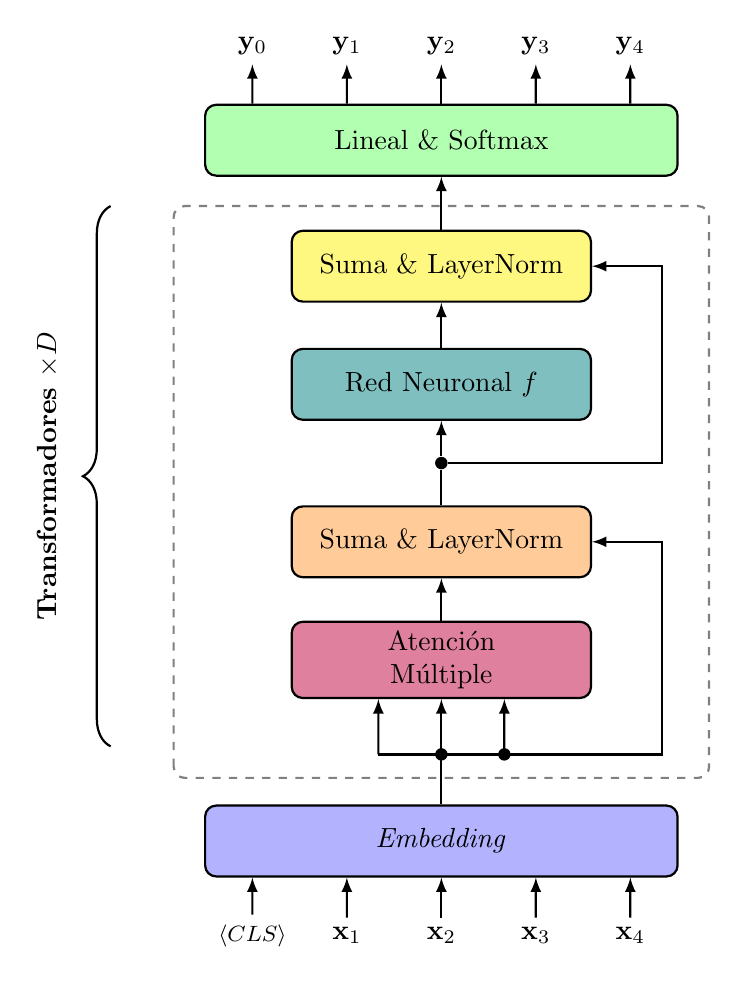
\begin{tikzpicture}[
        >=latex,
        box/.style={
            draw, thick, rounded corners=4pt, 
            minimum width=6cm, minimum height=0.9cm, 
            align=center
        },
        % Estilos de los bloques
        emb/.style={box, fill=blue!30},
        attn/.style={box, fill=purple!50, minimum width=3.8cm},
        addnorm/.style={box, fill=orange!40, minimum width=3.8cm},
        mlp/.style={box, fill=teal!50, minimum width=3.8cm},
        final/.style={box, fill=yellow!50, minimum width=3.8cm},
        % Ajustado a 6cm para igualar al Embedding
        outbox/.style={box, fill=green!30, minimum width=6cm},
        dot/.style={circle, fill=black, inner sep=0pt, minimum size=4.5pt}
    ]
    
    % 1. ENTRADAS (Tokens)
    \node[font=\footnotesize] (x_0) at (-2.4, 0) {$\langle CLS \rangle$};
    \node (x_1) at (-1.2, 0) {$\mathbf{x}_1$};
    \node (x_2) at (0, 0) {$\mathbf{x}_2$};
    \node (x_3) at (1.2, 0) {$\mathbf{x}_3$};
    \node (x_4) at (2.4, 0) {$\mathbf{x}_4$};
    
    % 2. BLOQUE EMBEDDING
    \node[emb] (emb) at (0, 1.2) {\textit{Embedding}};
    
    \draw[->, thick] (x_0) -- ([xshift=-2.4cm]emb.south);
    \draw[->, thick] (x_1) -- ([xshift=-1.2cm]emb.south);
    \draw[->, thick] (x_2) -- (emb.south);
    \draw[->, thick] (x_3) -- ([xshift=1.2cm]emb.south);
    \draw[->, thick] (x_4) -- ([xshift=2.4cm]emb.south);
    
    % 3. Bifurcación de entrada al Transformer
    \coordinate (c_center) at (0, 2.3);
    \coordinate (c_left) at (-0.8, 2.3);
    \coordinate (c_right) at (0.8, 2.3);
    
    \draw[thick] (emb.north) -- (c_center);
    \draw[thick] (c_center) -- (c_left);
    \draw[thick] (c_center) -- (c_right);
    \node[dot] at (c_center) {};
    \node[dot] at (c_right) {};
    
    % 4. BLOQUE DE ATENCIÓN
    \node[attn] (mha) at (0, 3.5) {Atención \\ Múltiple};
    \draw[->, thick] (c_center) -- (mha.south);
    \draw[->, thick] (c_left) -- ([xshift=-0.8cm]mha.south);
    \draw[->, thick] (c_right) -- ([xshift=0.8cm]mha.south);

    % 5. PRIMER ADD & NORM
    \node[addnorm] (an1) at (0, 5.0) {Suma \& LayerNorm};
    \draw[->, thick] (mha.north) -- (an1.south);
    \draw[->, thick] (c_right) -- (2.8, 2.3) |- (an1.east);
    
    % 6. PUNTO INTERMEDIO Z
    \coordinate (z_pos) at (0, 6.0);
    \node[dot] (dot_z) at (z_pos) {};
    \draw[thick] (an1.north) -- (dot_z);
    
    % 7. BLOQUE MLP
    \node[mlp] (mlp) at (0, 7.0) {Red Neuronal $f$};
    \draw[->, thick] (dot_z) -- (mlp.south);
    
    % 8. SEGUNDO ADD & NORM
    \node[final] (an2) at (0, 8.5) {Suma \& LayerNorm};
    \draw[->, thick] (mlp.north) -- (an2.south);
    \draw[->, thick] (dot_z) -- (2.8, 6.0) |- (an2.east);

    % --- RECUADRO DISCONTINUO ---
    \draw[dashed, thick, gray, rounded corners=4pt] 
        ([xshift=-3.4cm, yshift=-1cm]mha.south) 
        rectangle 
        ([xshift=3.4cm, yshift=0.3cm]an2.north);
        
    % --- LLAVE IZQUIERDA ---
    \draw[decorate, decoration={brace, amplitude=10pt}, thick] 
        ([xshift=-4.2cm, yshift=-0.6cm]mha.south) -- 
        ([xshift=-4.2cm, yshift=0.3cm]an2.north) 
        node[midway, xshift=-0.8cm, rotate=90, font=\bfseries] {Transformadores $\times D$};

    % 9. CAPA LINEAL & SOFTMAX (Ahora es de 6cm)
    \node[outbox] (soft) at (0, 10.1) {Lineal \& Softmax};
    \draw[->, thick] (an2.north) -- (soft.south);
    
    % 10. VECTORES DE SALIDA y_0 a y_4
    \node (y_0) at (-2.4, 11.3) {$\mathbf{y}_0$};
    \node (y_1) at (-1.2, 11.3) {$\mathbf{y}_1$};
    \node (y_2) at (0, 11.3) {$\mathbf{y}_2$};
    \node (y_3) at (1.2, 11.3) {$\mathbf{y}_3$};
    \node (y_4) at (2.4, 11.3) {$\mathbf{y}_4$};

    % Flechas directas desde Lineal & Softmax hacia los vectores y
    \draw[->, thick] ([xshift=-2.4cm]soft.north) -- (y_0);
    \draw[->, thick] ([xshift=-1.2cm]soft.north) -- (y_1);
    \draw[->, thick] (soft.north) -- (y_2);
    \draw[->, thick] ([xshift=1.2cm]soft.north) -- (y_3);
    \draw[->, thick] ([xshift=2.4cm]soft.north) -- (y_4);
    
    \end{tikzpicture}
}

\newcommand{\DiagramaCodificadorFT}{
    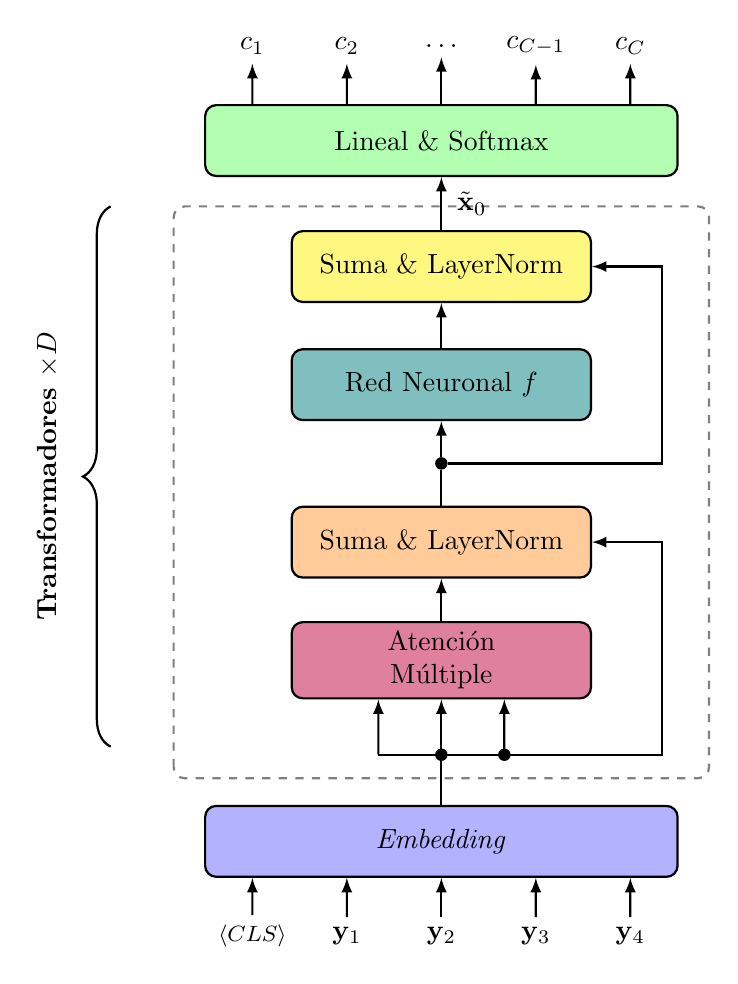
\begin{tikzpicture}[
        >=latex,
        box/.style={
            draw, thick, rounded corners=4pt, 
            minimum width=6cm, minimum height=0.9cm, 
            align=center
        },
        % Estilos de los bloques
        emb/.style={box, fill=blue!30},
        attn/.style={box, fill=purple!50, minimum width=3.8cm},
        addnorm/.style={box, fill=orange!40, minimum width=3.8cm},
        mlp/.style={box, fill=teal!50, minimum width=3.8cm},
        final/.style={box, fill=yellow!50, minimum width=3.8cm},
        outbox/.style={box, fill=green!30, minimum width=6cm},
        dot/.style={circle, fill=black, inner sep=0pt, minimum size=4.5pt}
    ]
    
    % 1. ENTRADAS (Tokens)
    \node[font=\footnotesize] (x_0) at (-2.4, 0) {$\langle CLS \rangle$};
    \node (x_1) at (-1.2, 0) {$\mathbf{y}_1$};
    \node (x_2) at (0, 0) {$\mathbf{y}_2$};
    \node (x_3) at (1.2, 0) {$\mathbf{y}_3$};
    \node (x_4) at (2.4, 0) {$\mathbf{y}_4$};
    
    % 2. BLOQUE EMBEDDING
    \node[emb] (emb) at (0, 1.2) {\textit{Embedding}};
    
    \draw[->, thick] (x_0) -- ([xshift=-2.4cm]emb.south);
    \draw[->, thick] (x_1) -- ([xshift=-1.2cm]emb.south);
    \draw[->, thick] (x_2) -- (emb.south);
    \draw[->, thick] (x_3) -- ([xshift=1.2cm]emb.south);
    \draw[->, thick] (x_4) -- ([xshift=2.4cm]emb.south);
    
    % 3. Bifurcación de entrada al Transformer
    \coordinate (c_center) at (0, 2.3);
    \coordinate (c_left) at (-0.8, 2.3);
    \coordinate (c_right) at (0.8, 2.3);
    
    \draw[thick] (emb.north) -- (c_center);
    \draw[thick] (c_center) -- (c_left);
    \draw[thick] (c_center) -- (c_right);
    \node[dot] at (c_center) {};
    \node[dot] at (c_right) {};
    
    % 4. BLOQUE DE ATENCIÓN
    \node[attn] (mha) at (0, 3.5) {Atención \\ Múltiple};
    \draw[->, thick] (c_center) -- (mha.south);
    \draw[->, thick] (c_left) -- ([xshift=-0.8cm]mha.south);
    \draw[->, thick] (c_right) -- ([xshift=0.8cm]mha.south);

    % 5. PRIMER ADD & NORM
    \node[addnorm] (an1) at (0, 5.0) {Suma \& LayerNorm};
    \draw[->, thick] (mha.north) -- (an1.south);
    \draw[->, thick] (c_right) -- (2.8, 2.3) |- (an1.east);
    
    % 6. PUNTO INTERMEDIO Z
    \coordinate (z_pos) at (0, 6.0);
    \node[dot] (dot_z) at (z_pos) {};
    \draw[thick] (an1.north) -- (dot_z);
    
    % 7. BLOQUE MLP
    \node[mlp] (mlp) at (0, 7.0) {Red Neuronal $f$};
    \draw[->, thick] (dot_z) -- (mlp.south);
    
    % 8. SEGUNDO ADD & NORM
    \node[final] (an2) at (0, 8.5) {Suma \& LayerNorm};
    \draw[->, thick] (mlp.north) -- (an2.south);
    \draw[->, thick] (dot_z) -- (2.8, 6.0) |- (an2.east);

    % --- RECUADRO DISCONTINUO ---
    \draw[dashed, thick, gray, rounded corners=4pt] 
        ([xshift=-3.4cm, yshift=-1cm]mha.south) 
        rectangle 
        ([xshift=3.4cm, yshift=0.3cm]an2.north);
        
    % --- LLAVE IZQUIERDA ---
    \draw[decorate, decoration={brace, amplitude=10pt}, thick] 
        ([xshift=-4.2cm, yshift=-0.6cm]mha.south) -- 
        ([xshift=-4.2cm, yshift=0.3cm]an2.north) 
        node[midway, xshift=-0.8cm, rotate=90, font=\bfseries] {Transformadores $\times D$};

    % 9. CAPA LINEAL & SOFTMAX con etiqueta x_0 tilde
    \node[outbox] (soft) at (0, 10.1) {Lineal \& Softmax};
    \draw[->, thick] (an2.north) -- (soft.south) node[midway, right, xshift=2pt] {$\tilde{\mathbf{x}}_0$};
    
    % 10. VECTORES DE SALIDA c_1 ... c_C
    \node (c_1) at (-2.4, 11.3) {$c_1$};
    \node (c_2) at (-1.2, 11.3) {$c_2$};
    \node (dots) at (0, 11.3) {$\dots$};
    \node (c_prev) at (1.2, 11.3) {$c_{C-1}$};
    \node (c_C) at (2.4, 11.3) {$c_C$};

    % Flechas directas desde Lineal & Softmax hacia los resultados c
    \draw[->, thick] ([xshift=-2.4cm]soft.north) -- (c_1);
    \draw[->, thick] ([xshift=-1.2cm]soft.north) -- (c_2);
    \draw[->, thick] (soft.north) -- (dots);
    \draw[->, thick] ([xshift=1.2cm]soft.north) -- (c_prev);
    \draw[->, thick] ([xshift=2.4cm]soft.north) -- (c_C);
    
    \end{tikzpicture}
}
%===========================
%CODIFICADOR-DECODIFICADOR
%===========================
\newcommand{\DiagramaCodificadorDecodificador}{
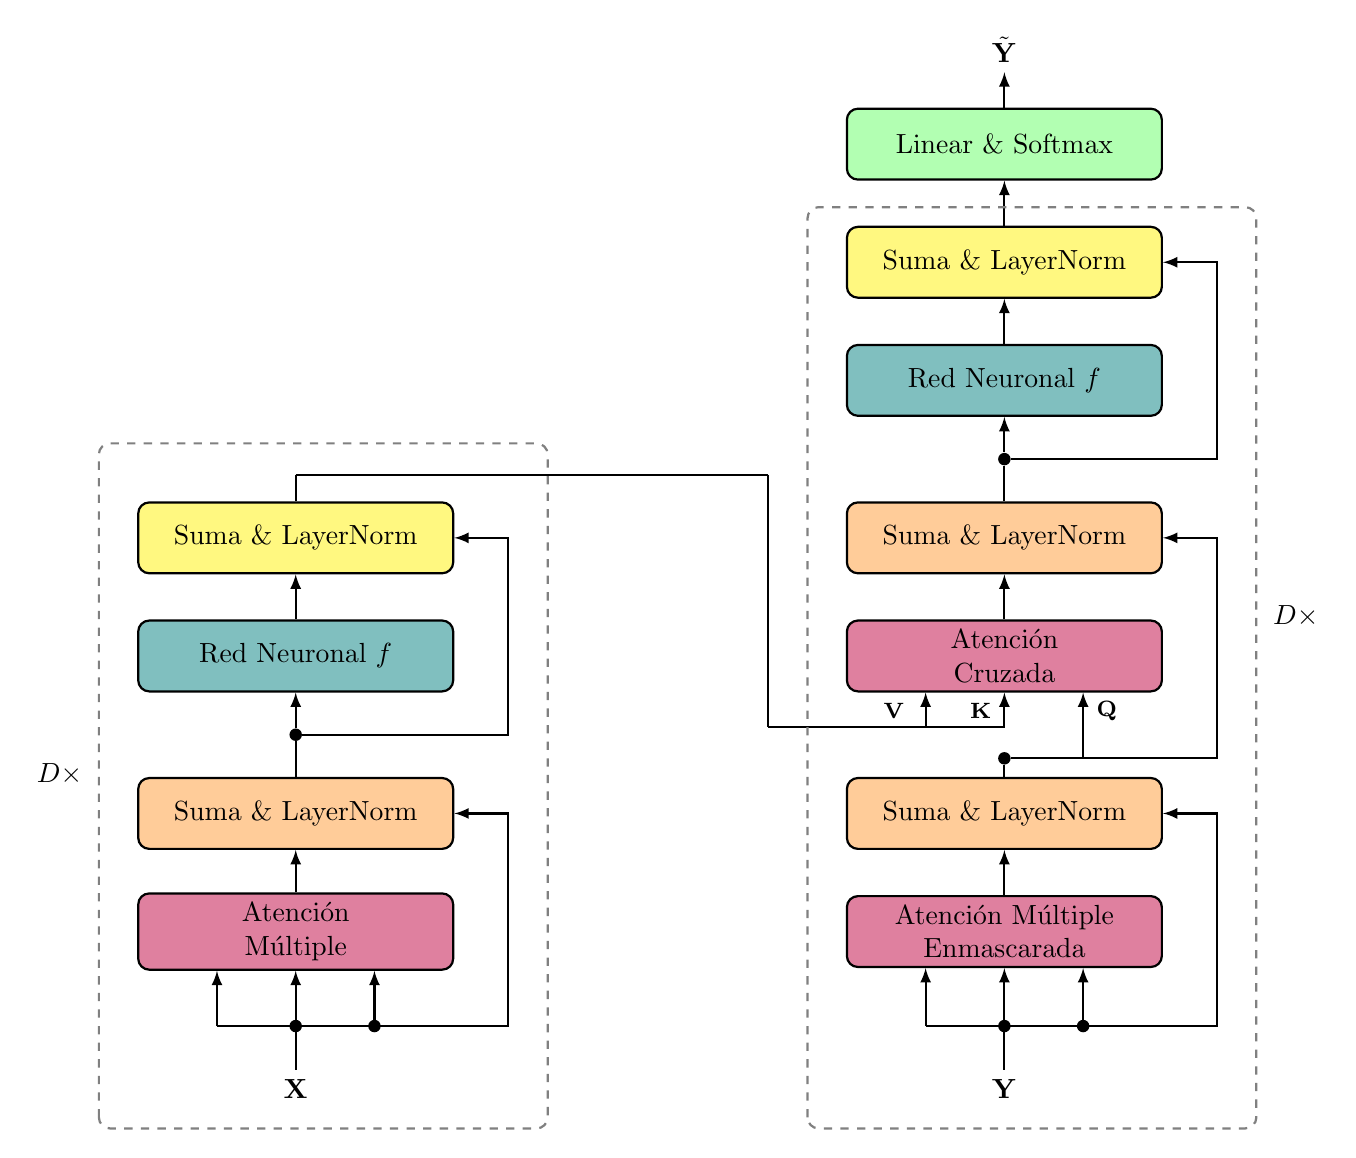
\begin{tikzpicture}[
        >=latex,
        box/.style={
            draw, thick, rounded corners=4pt, 
            minimum width=4.0cm, minimum height=0.9cm, 
            align=center
        },
        attn/.style={box, fill=purple!50},
        addnorm/.style={box, fill=orange!40},
        mlp/.style={box, fill=teal!50},
        dot/.style={circle, fill=black, inner sep=0pt, minimum size=4.5pt},
        final/.style={box, fill=yellow!50},
        outbox/.style={box, fill=green!30} % Nuevo estilo para Linear & Softmax
    ]

    % ==========================================
    % 1. CODIFICADOR (Lado Izquierdo)
    % ==========================================
    \coordinate (enc_x) at (-4.5, 0);
    \node (x) at (enc_x) {$\mathbf{X}$};

    % Bloque de Atención Múltiple
    \node[attn] (e_mha) at (-4.5, 2) {Atención \\ Múltiple};
    
    % Bifurcaciones entrada
    \coordinate (e_c_center) at (-4.5, 0.8);
    \coordinate (e_c_left) at (-5.5, 0.8);
    \coordinate (e_c_right) at (-3.5, 0.8);

    \draw[thick] (x) -- (e_c_center);
    \draw[thick] (e_c_center) -- (e_c_left);
    \draw[thick] (e_c_center) -- (e_c_right);

    \node[dot] at (e_c_center) {};
    \node[dot] at (e_c_right) {};

    % Flechas hacia la atención
    \draw[->, thick] (e_c_center) -- (e_mha.south);
    \draw[->, thick] (e_c_left) -- ([xshift=-1cm]e_mha.south);
    \draw[->, thick] (e_c_right) -- ([xshift=1cm]e_mha.south);

    % Primer Add & Norm
    \node[addnorm] (e_an1) at (-4.5, 3.5) {Suma \& LayerNorm};
    \draw[->, thick] (e_mha.north) -- (e_an1.south);

    % Primera conexión residual del Codificador
    \draw[->, thick] (e_c_right) -- (-1.8, 0.8) |- (e_an1.east);

    % Variable intermedia
    \coordinate (e_z1_pos) at (-4.5, 4.5);
    \node[dot] (e_dot_z1) at (e_z1_pos) {};
    \draw[thick] (e_an1.north) -- (e_dot_z1);

    % Bloque MLP
    \node[mlp] (e_mlp) at (-4.5, 5.5) {Red Neuronal $f$};
    \draw[->, thick] (e_dot_z1) -- (e_mlp.south);

    % Segundo Add & Norm
    \node[final] (e_an2) at (-4.5, 7.0) {Suma \& LayerNorm};
    \draw[->, thick] (e_mlp.north) -- (e_an2.south);

    % Segunda conexión residual del Codificador
    \draw[->, thick] (e_dot_z1) -- (-1.8, 4.5) |- (e_an2.east);

    % Recuadro y Título del Codificador
    \draw[dashed, gray, thick, rounded corners] (-7.0, -0.5) rectangle (-1.3, 8.2);
    \node (N_1) at (-7.5,4) {$D \times $};
    


    % ==========================================
    % 2. DECODIFICADOR (Lado Derecho)
    % ==========================================
    \coordinate (dec_x) at (4.5, 0);
    \node (y) at (dec_x) {$\mathbf{Y}$};

    % Atención Enmascarada
    \node[attn] (d_mmha) at (4.5, 2) {Atención Múltiple \\ Enmascarada};

    % Bifurcaciones entrada
    \coordinate (d_c_center) at (4.5, 0.8);
    \coordinate (d_c_left) at (3.5, 0.8);
    \coordinate (d_c_right) at (5.5, 0.8);

    \draw[thick] (y) -- (d_c_center);
    \draw[thick] (d_c_center) -- (d_c_left);
    \draw[thick] (d_c_center) -- (d_c_right);

    \node[dot] at (d_c_center) {};
    \node[dot] at (d_c_right) {};

    \draw[->, thick] (d_c_center) -- (d_mmha.south);
    \draw[->, thick] (d_c_left) -- ([xshift=-1cm]d_mmha.south);
    \draw[->, thick] (d_c_right) -- ([xshift=1cm]d_mmha.south);

    % Primer Add & Norm
    \node[addnorm] (d_an1) at (4.5, 3.5) {Suma \& LayerNorm};
    \draw[->, thick] (d_mmha.north) -- (d_an1.south);

    % Primera conexión residual del Decodificador
    \draw[->, thick] (d_c_right) -- (7.2, 0.8) |- (d_an1.east);

    % ==========================================
    % 3. ATENCIÓN CRUZADA (Cross-Attention)
    % ==========================================
    \node[attn] (d_cross) at (4.5, 5.5) {Atención \\ Cruzada};
    
    % Conexión Q desde la capa anterior del Decodificador
    \coordinate (d_q_pos) at (4.5, 4.2);
    \node[dot] (d_dot_q) at (d_q_pos) {};
    \draw[thick] (d_an1.north) -- (d_dot_q);
    % Q entra por la derecha (consulta)
    \draw[->, thick] (d_dot_q) -- (5.5, 4.2) -- ([xshift=1cm]d_cross.south);

    % Conexiones K y V desde la salida del Codificador
    \coordinate (e_out) at (-4.5, 7.8);
    \draw[thick] (e_an2.north) -- (e_out);
    
    % Trazado de la línea principal desde Codificador a Decodificador
    \coordinate (cross_split) at (1.5, 7.8);
    \draw[thick] (e_out) -- (cross_split);
    \coordinate (cross_drop) at (1.5, 4.6);
    \draw[thick] (cross_split) -- (cross_drop);
    %\node[dot] at (cross_drop) {};

    % V va a la izquierda
    \draw[->, thick] (cross_drop) -- (3.5, 4.6) -- ([xshift=-1cm]d_cross.south);
    % K va al centro
    \draw[->, thick] (cross_drop) -- (4.5, 4.6) -- (d_cross.south);

    % Etiquetas K, V, Q para mayor claridad
    \node[font=\footnotesize] at (3.1, 4.8) {$\mathbf{V}$};
    \node[font=\footnotesize] at (4.2, 4.8) {$\mathbf{K}$};
    \node[font=\footnotesize] at (5.8, 4.8) {$\mathbf{Q}$};

    % ==========================================
    % 4. RESTO DEL DECODER Y NUEVA SALIDA
    % ==========================================
    % Segundo Add & Norm
    \node[addnorm] (d_an2) at (4.5, 7.0) {Suma \& LayerNorm};
    \draw[->, thick] (d_cross.north) -- (d_an2.south);

    % Segunda conexión residual del Decodificador (viene de Q)
    \draw[->, thick] (d_dot_q) -- (7.2, 4.2) |- (d_an2.east);

    % Variable intermedia Z del decoder
    \coordinate (d_z3_pos) at (4.5, 8.0);
    \node[dot] (d_dot_z3) at (d_z3_pos) {};
    \draw[thick] (d_an2.north) -- (d_dot_z3);

    % Bloque MLP
    \node[mlp] (d_mlp) at (4.5, 9.0) {Red Neuronal $f$};
    \draw[->, thick] (d_dot_z3) -- (d_mlp.south);

    % Tercer Add & Norm
    \node[final] (d_an3) at (4.5, 10.5) {Suma \& LayerNorm};
    \draw[->, thick] (d_mlp.north) -- (d_an3.south);

    % Tercera conexión residual del Decodificador
    \draw[->, thick] (d_dot_z3) -- (7.2, 8.0) |- (d_an3.east);

    % --- NUEVA CAPA: Linear & Softmax ---
    \node[outbox] (d_linsoft) at (4.5, 12.0) {Linear \& Softmax};
    \draw[->, thick] (d_an3.north) -- (d_linsoft.south);

    % Salida final Decoder
    \node (ytilde) at (4.5, 13.2) {$\tilde{\mathbf{Y}}$};
    \draw[->, thick] (d_linsoft.north) -- (ytilde);

    % Recuadro y Título del Decodificador (Altura ajustada para incluir Linear & Softmax)
    \draw[dashed, gray, thick, rounded corners] (2, -0.5) rectangle (7.7, 11.2);
    \node (N_2) at (8.2,6) {$D \times $};

\end{tikzpicture}
}


%===========================
%BPE
%===========================
\newcommand{\BPE}{
Hoy ya es ayer y ayer ya es hoy, ya llegó el día, y hoy es hoy

H\textcolor{red}{\underline{oy}} ya es ayer y ayer ya es h\textcolor{red}{\underline{oy}}, ya llegó el día, y h\textcolor{red}{\underline{oy}} es h\textcolor{red}{\underline{oy}}

H\textcolor{red}{oy} ya \textcolor{orange}{\underline{es}} ayer y ayer ya \textcolor{orange}{\underline{es}} h\textcolor{red}{oy}, ya llegó el día, y h\textcolor{red}{oy} \textcolor{orange}{\underline{es}} h\textcolor{red}{oy}

H\textcolor{red}{oy} ya \textcolor{orange}{es} ayer y ayer ya \textcolor{orange}{es} \textcolor{teal!50}{\underline{hoy}}, ya llegó el día, y \textcolor{teal!50}{\underline{hoy}} \textcolor{orange}{es} \textcolor{teal!50}{\underline{hoy}}


H\textcolor{red}{oy} \textcolor{purple!50}{\underline{ya}} \textcolor{orange}{es} ayer y ayer \textcolor{purple!50}{\underline{ya}}  \textcolor{orange}{es} \textcolor{teal!50}{hoy}, \textcolor{purple!50}{\underline{ya}}  llegó el día, y \textcolor{teal!50}{hoy} \textcolor{orange}{es} \textcolor{teal!50}{hoy}
}

%==============================
%ENCODER MASK
%==============================





